\chapter{QFT-96 focused results and run ledger}
\label{ch:qft96-focus}

This chapter is the single location for the current QFT-96 investigation. It
is intentionally separate from the historical multi-workload chapters. QFT-96
is a 96-logical-qubit, 766-layer circuit generated by the mapper workflow and
placed with T-HQA at mapping seeds 42, 43 and 44. The original logical
migrations are held fixed when comparing routing and topology: mesh uses XY,
YX, shortest-reliable and maximum-reliability; torus uses Dijkstra only.

The route exporter validated all 15 conceptual route artifacts for migration
endpoints, adjacent-hop validity, trace hashes and replay to the placement.
There are 11 byte-distinct traces after exact deduplication. The base ACE phase
enumerates memories $M\in\{2,3,4,6,8,16,32,64\}$, every legal compiler
allocation $C=0,\ldots,M-1$, ODG, CGP, ACGP, Dynamic full-chain and Dynamic
first-hop, with physics seeds 0 and 1. A separate Dynamic-policy phase fixes
$M=4$, $C=3$ and evaluates the 13 launch-policy variants listed in the research
ledger. All timing uses the corrected arrival-to-completion simulator metric;
the historical 5.3-ms subtraction is not used.

\section{Progress snapshot}

The following ledger is a snapshot at this PDF build. A directory is counted
only after its execution record, metadata, input hashes, seed rows and 100\%
completion have validated. Counts are expected to increase while the runners
remain active; they must not be read as final results.

\begin{table}[H]
\centering\small
\caption{QFT-96-only execution ledger at build time. Exact manifests and raw outputs are linked in the repository.}
\label{tab:qft96-ledger}
\begin{tabular}{p{0.30\linewidth}r r p{0.34\linewidth}}
\toprule
Phase & Validated jobs & Planned jobs & Status and source artifacts \\
\midrule
Mapper and route audit & 15 & 15 & Complete; mapping audit CSV and route traces \\
Base ACE matrix & 71 & 3,058 & Running; base-evaluation manifest and progress CSV \\
Dynamic launch variants & 10 & 143 & Running; dynamic-variants manifest \\
Four-memory matched checkpoint & 10 cells & 10 cells & Complete; checkpoint CSV and seed CSV \\
\bottomrule
\end{tabular}
\end{table}

The authoritative QFT-96 study root is
\href{https://github.com/sanjeevkrishnaa/Compiler-Driven-ACE/tree/codex/ace-scheduler-correctness/results/qft96_2seed_2026-10-26}{\texttt{results/qft96\_2seed\_2026-10-26}}.
The base plan is in
\href{https://github.com/sanjeevkrishnaa/Compiler-Driven-ACE/blob/codex/ace-scheduler-correctness/results/qft96_2seed_2026-10-26/manifests/base-evaluation\_jobs.jsonl.gz}{the base manifest}; the Dynamic-policy plan is in
\href{https://github.com/sanjeevkrishnaa/Compiler-Driven-ACE/blob/codex/ace-scheduler-correctness/results/qft96_2seed_2026-10-26/manifests/dynamic-variants\_jobs.json}{the variant manifest}.

\section{Validated route structure}

% Generated by tools/golden_study/plot_qft96_routes.py; do not edit by hand.
\begin{figure}[H]
\centering
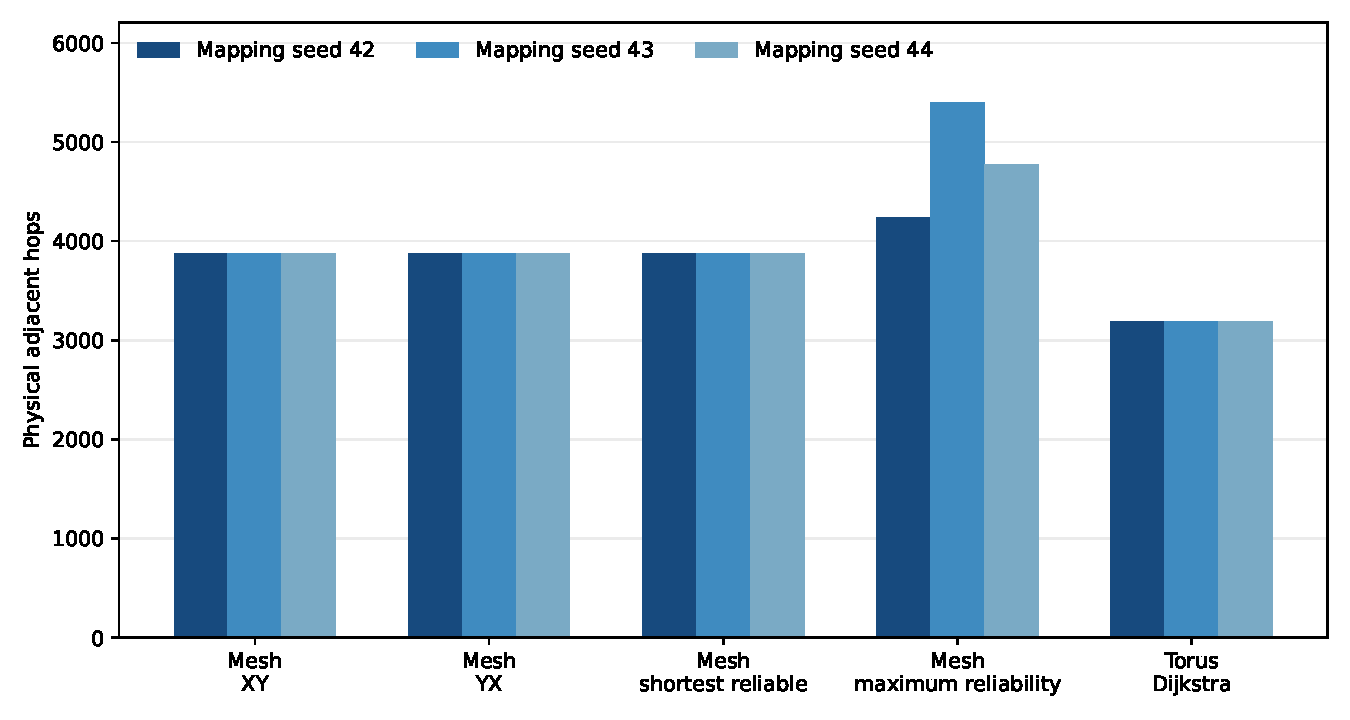
\includegraphics[width=0.78\linewidth]{../../../results/qft96_2seed_2026-10-26/figures/qft96_route_hops.pdf}
\caption{QFT-96 adjacent-hop count on the same T-HQA placement for each seed. Torus uses Dijkstra. These are structural counts, not simulated latency. The complete values are in Table~\ref{tab:qft96-route-hops} and the \href{https://github.com/sanjeevkrishnaa/Compiler-Driven-ACE/blob/codex/ace-scheduler-correctness/results/qft96_2seed_2026-10-26/validation/mapping_audit.csv}{source CSV}.}
\label{fig:qft96-route-hops}
\end{figure}
\begin{table}[H]
\centering\small
\begin{tabular}{lrrr}
\toprule
Route & Seed 42 hops & Seed 43 hops & Seed 44 hops \\
\midrule
Mesh XY & 3876 & 3876 & 3876 \\
Mesh YX & 3876 & 3876 & 3876 \\
Mesh shortest reliable & 3876 & 3876 & 3876 \\
Mesh maximum reliability & 4242 & 5396 & 4774 \\
Torus Dijkstra & 3186 & 3186 & 3186 \\
\bottomrule
\end{tabular}
\caption{Exact QFT-96 route counts for all three mapping seeds. Every row has 1,965 logical migrations and 766 layers. \href{https://github.com/sanjeevkrishnaa/Compiler-Driven-ACE/blob/codex/ace-scheduler-correctness/results/qft96_2seed_2026-10-26/validation/mapping_audit.csv}{Source CSV}.}
\label{tab:qft96-route-hops}
\end{table}


The route-count figure is structural only. It does not replace simulator
latency, admission wait, makespan, fidelity or waste measurements.

\section{Validated four-memory checkpoint}

The first complete timing checkpoint fixes four shared memories per core, three
compiler memories for pre-generation, mapping seed 42, and physics seeds 0 and
1. It compares the same QFT-96 logical migration sequence under mesh XY and
torus Dijkstra. It is useful for validating the pipeline, but it is not the
final memory/routing/policy ranking.

% Generated by tools/golden_study/plot_qft96_checkpoint.py; do not edit by hand.
\begin{figure}[H]
\centering
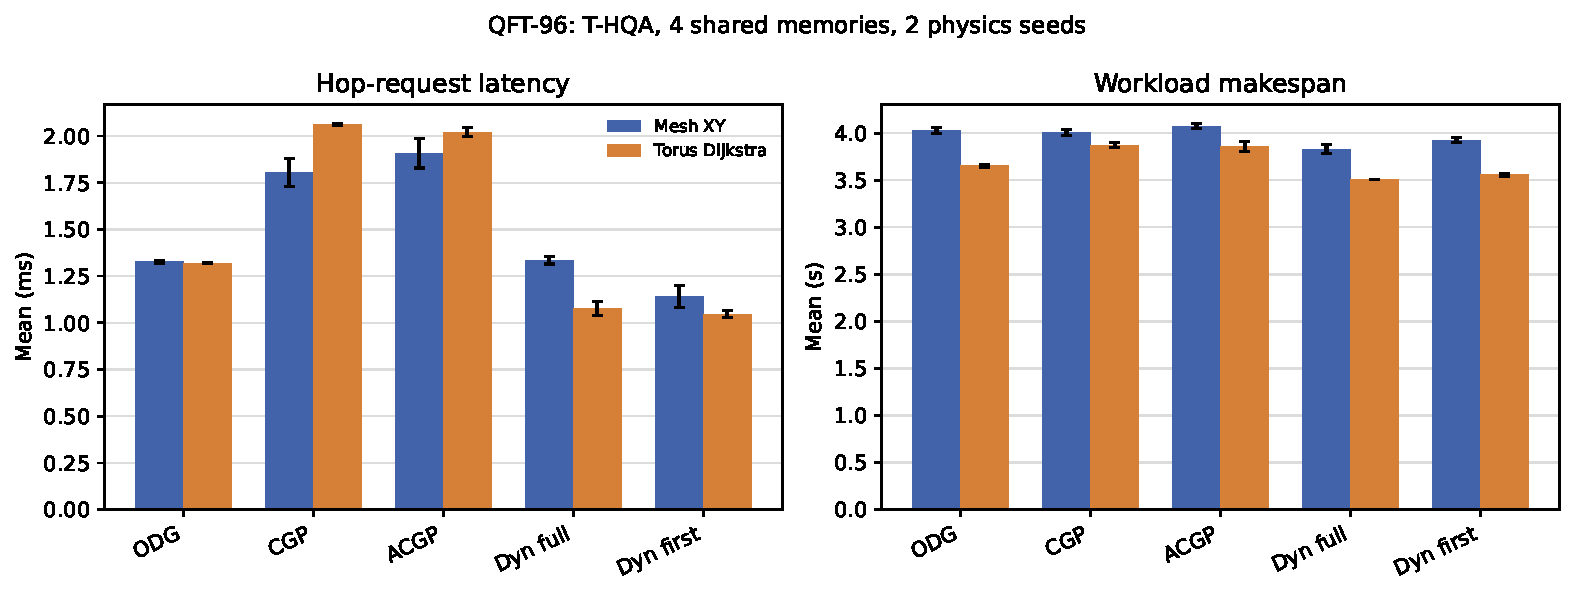
\includegraphics[width=0.9\linewidth]{../../../results/qft96_2seed_2026-10-26/figures/qft96_m4_checkpoint.pdf}
\caption{Validated QFT-96 four-memory checkpoint. Bars show means and standard deviations across physics seeds 0 and 1, not uncertainty across mapping placements. Mesh XY and torus Dijkstra use the same logical migration endpoints. Exact values are in Table~\ref{tab:qft96-m4-timing} and the \href{https://github.com/sanjeevkrishnaa/Compiler-Driven-ACE/blob/codex/ace-scheduler-correctness/results/qft96_2seed_2026-10-26/summaries/qft96_m4_checkpoint.csv}{aggregate CSV}; \href{https://github.com/sanjeevkrishnaa/Compiler-Driven-ACE/blob/codex/ace-scheduler-correctness/results/qft96_2seed_2026-10-26/summaries/qft96_m4_seed_rows.csv}{per-seed rows} are also archived.}
\label{fig:qft96-m4-checkpoint}
\end{figure}
\begin{table}[H]
\centering\scriptsize
\begin{tabular}{llrrrr}
\toprule
Route & Policy & Latency (ms) & p95 (ms) & Makespan (s) & Admission (ms) \\
\midrule
Mesh XY & ODG & 1.327 $\pm$ 0.006 & 3.100 & 4.033 $\pm$ 0.031 & 0.008 \\
Mesh XY & CGP & 1.803 $\pm$ 0.075 & 5.150 & 4.006 $\pm$ 0.031 & 1.043 \\
Mesh XY & ACGP & 1.908 $\pm$ 0.079 & 5.600 & 4.075 $\pm$ 0.028 & 1.149 \\
Mesh XY & Dyn full & 1.335 $\pm$ 0.020 & 4.050 & 3.830 $\pm$ 0.048 & 0.551 \\
Mesh XY & Dyn first-hop & 1.141 $\pm$ 0.058 & 2.900 & 3.928 $\pm$ 0.029 & 0.125 \\
Torus Dijkstra & ODG & 1.320 $\pm$ 0.002 & 3.000 & 3.654 $\pm$ 0.013 & 0.004 \\
Torus Dijkstra & CGP & 2.061 $\pm$ 0.006 & 5.400 & 3.874 $\pm$ 0.024 & 1.223 \\
Torus Dijkstra & ACGP & 2.021 $\pm$ 0.023 & 5.300 & 3.855 $\pm$ 0.054 & 1.199 \\
Torus Dijkstra & Dyn full & 1.075 $\pm$ 0.037 & 2.900 & 3.509 $\pm$ 0.000 & 0.328 \\
Torus Dijkstra & Dyn first-hop & 1.046 $\pm$ 0.019 & 2.700 & 3.557 $\pm$ 0.013 & 0.132 \\
\bottomrule
\end{tabular}
\caption{Complete matched timing values for Figure~\ref{fig:qft96-m4-checkpoint}. ODG has $C=0$; other policies have $C=3$. Latency and makespan show mean $\pm$ sample SD across two physics seeds. The full precision and raw job identifiers are in the \href{https://github.com/sanjeevkrishnaa/Compiler-Driven-ACE/blob/codex/ace-scheduler-correctness/results/qft96_2seed_2026-10-26/summaries/qft96_m4_checkpoint.csv}{source CSV}.}
\label{tab:qft96-m4-timing}
\end{table}
\begin{table}[H]
\centering\scriptsize
\begin{tabular}{llrrr}
\toprule
Route & Policy & Pre-generated hit rate & Protocol waste (\%) & Fidelity \\
\midrule
Mesh XY & ODG & N/A & N/A & 0.9498 \\
Mesh XY & CGP & N/A & 15.07 & 0.9271 \\
Mesh XY & ACGP & N/A & 15.27 & 0.9262 \\
Mesh XY & Dyn full & 0.602 & 0.00 & 0.9438 \\
Mesh XY & Dyn first-hop & 0.340 & 0.00 & 0.9472 \\
Torus Dijkstra & ODG & N/A & N/A & 0.9498 \\
Torus Dijkstra & CGP & N/A & 19.74 & 0.9311 \\
Torus Dijkstra & ACGP & N/A & 19.14 & 0.9307 \\
Torus Dijkstra & Dyn full & 0.656 & 0.00 & 0.9440 \\
Torus Dijkstra & Dyn first-hop & 0.455 & 0.00 & 0.9462 \\
\bottomrule
\end{tabular}
\caption{Readiness, waste and delivered-pair fidelity for the same validated checkpoint; ODG has no pre-generated cache. \href{https://github.com/sanjeevkrishnaa/Compiler-Driven-ACE/blob/codex/ace-scheduler-correctness/results/qft96_2seed_2026-10-26/summaries/qft96_m4_checkpoint.csv}{Source CSV}.}
\label{tab:qft96-m4-quality}
\end{table}


\section{Interpretation boundary}

No claim that Dynamic is generally better is made from the checkpoint or from
the partial ledger. Final conclusions require all base cells and all 13
launch-policy variants to validate. The separate congestion-adaptive Dynamic
policy is not silently folded into this phase: it requires a QFT-96-specific
training split and a frozen threshold before evaluation. When that training
phase is complete, its manifest and results will be added here as another
explicit row rather than changing the meaning of existing rows.

\section{Reproduction links}

The exact summary and per-seed CSVs are preserved under the QFT-96 study root:
\begin{itemize}
\item \href{https://github.com/sanjeevkrishnaa/Compiler-Driven-ACE/blob/codex/ace-scheduler-correctness/results/qft96_2seed_2026-10-26/validation/mapping_audit.csv}{mapping audit CSV};
\item \href{https://github.com/sanjeevkrishnaa/Compiler-Driven-ACE/blob/codex/ace-scheduler-correctness/results/qft96_2seed_2026-10-26/summaries/base-evaluation-progress.csv}{base progress CSV};
\item \href{https://github.com/sanjeevkrishnaa/Compiler-Driven-ACE/blob/codex/ace-scheduler-correctness/results/qft96_2seed_2026-10-26/summaries/qft96_m4_checkpoint.csv}{four-memory checkpoint CSV};
\item \href{https://github.com/sanjeevkrishnaa/Compiler-Driven-ACE/blob/codex/ace-scheduler-correctness/results/qft96_2seed_2026-10-26/summaries/qft96_m4_seed_rows.csv}{checkpoint per-seed CSV}.
\end{itemize}
